\documentclass[11pt]{article}
\usepackage{graphicx}
\usepackage{hyperref}
\usepackage{appendix}
\usepackage{amsmath}
\usepackage{amsthm}
\usepackage{amssymb}
\usepackage{float}
\usepackage{multirow}
\usepackage{commath}
\usepackage{booktabs}
\renewcommand{\arraystretch}{1.2}
\usepackage{siunitx}
\sisetup{detect-all}
\usepackage{listings}
\usepackage{color} %red, green, blue, yellow, cyan, magenta, black, white
\definecolor{mygreen}{RGB}{28,172,0} % color values Red, Green, Blue
\definecolor{mylilas}{RGB}{170,55,241}
\usepackage[a4paper,margin=20mm]{geometry}
\numberwithin{equation}{section}
\setlength{\parskip}{\baselineskip}
\setlength{\parindent}{0pt}
\hypersetup{
    colorlinks=true,
    linkcolor=black,
    filecolor=black,      
    urlcolor=black,
    citecolor=black
}
\urlstyle{same}
\begin{document}
\title{\textbf{UCL Mechanical Engineering 2020/2021}\\MECH0011 Final Coursework}
\author{NCWT3}
\maketitle
\tableofcontents
\listoffigures
\section{Question 1}
\subsection{a}
The data was imported into MATLAB and the shape of the hydrofoil, the chord line and the mean camber line were plotted for all four hydrofoils.
\lstset{language=Matlab,%
    %basicstyle=\color{red},
    breaklines=true,%
    morekeywords={matlab2tikz},
    keywordstyle=\color{blue},%
    morekeywords=[2]{1}, keywordstyle=[2]{\color{black}},
    identifierstyle=\color{black},%
    stringstyle=\color{mylilas},
    commentstyle=\color{mygreen},%
    showstringspaces=false,%without this there will be a symbol in the places where there is a space
    numbers=left,%
    numberstyle={\tiny \color{black}},% size of the numbers
    numbersep=9pt, % this defines how far the numbers are from the text
    emph=[1]{for,end,break},emphstyle=[1]\color{red}, %some words to emphasise
    %emph=[2]{word1,word2}, emphstyle=[2]{style},    
}
\lstinputlisting{./mCode/q1a.m}
\begin{figure}[H]
    \centering
    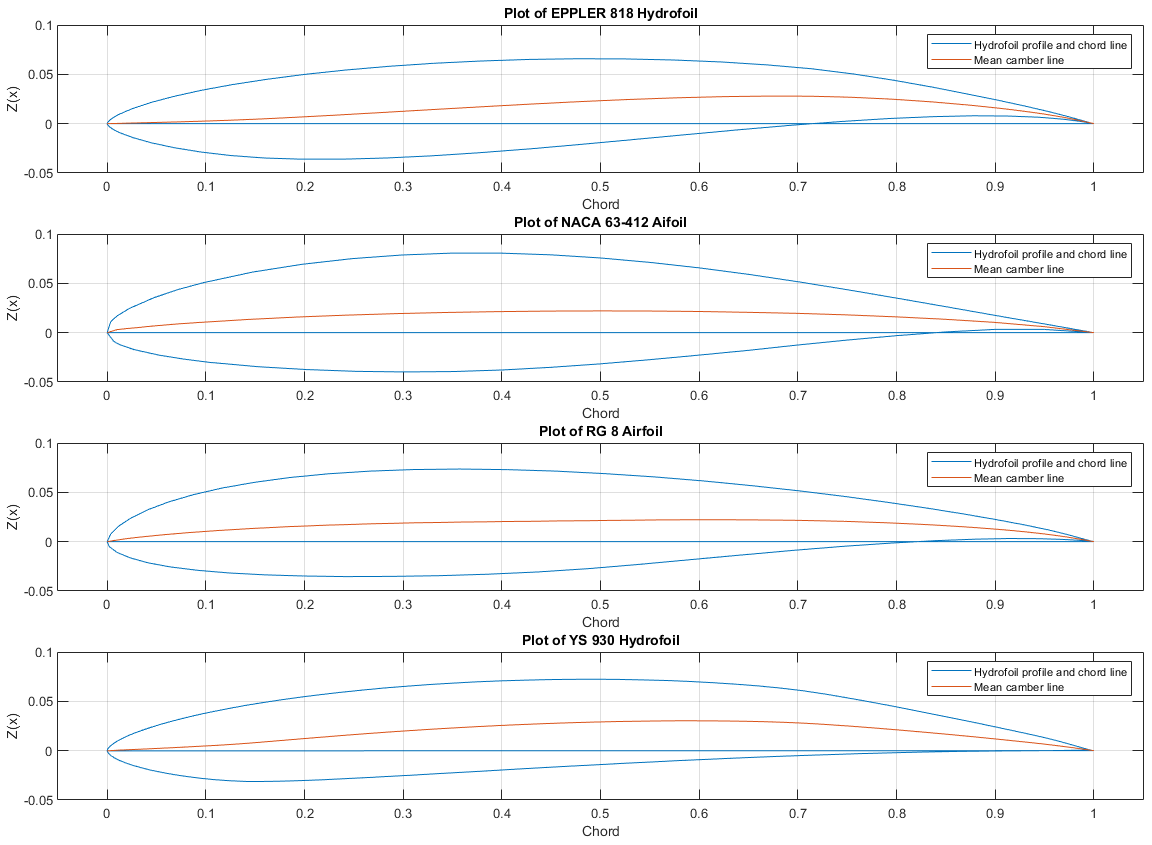
\includegraphics[width = \textwidth]{./img/q1a.png}
    \caption{Graphs to show hydrofoil shape, chord line and mean camber line for four different hydrofoils.}
    \label{fig:q1a}
\end{figure}
\subsection{b}
MATLAB was used to calculate the lift-to-drag ratio for each hydrofoil.
\lstset{language=Matlab,%
    %basicstyle=\color{red},
    breaklines=true,%
    morekeywords={matlab2tikz},
    keywordstyle=\color{blue},%
    morekeywords=[2]{1}, keywordstyle=[2]{\color{black}},
    identifierstyle=\color{black},%
    stringstyle=\color{mylilas},
    commentstyle=\color{mygreen},%
    showstringspaces=false,%without this there will be a symbol in the places where there is a space
    numbers=left,%
    numberstyle={\tiny \color{black}},% size of the numbers
    numbersep=9pt, % this defines how far the numbers are from the text
    emph=[1]{for,end,break},emphstyle=[1]\color{red}, %some words to emphasise
    %emph=[2]{word1,word2}, emphstyle=[2]{style},    
}
\lstinputlisting{./mCode/q1b.m}
\begin{figure}[H]
    \centering
    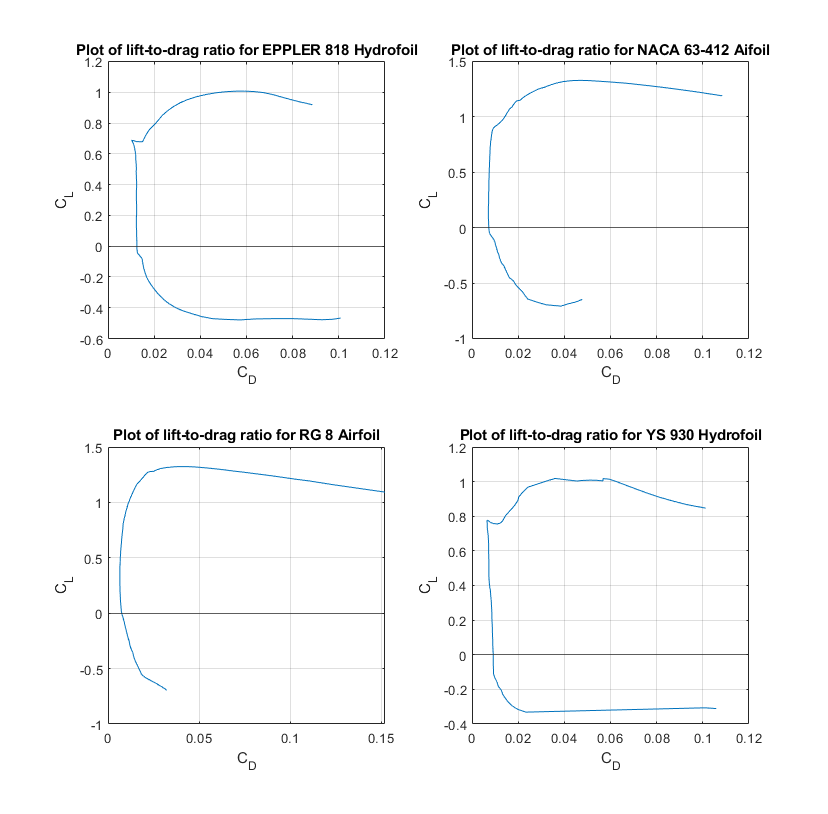
\includegraphics[width = \textwidth]{./img/q1b.png}
    \caption{Graphs to show lift-to-drag ratio for four different hydrofoils.}
    \label{fig:q1b}
\end{figure}
\subsection{c}
\subsection{d}
MATLAB was used to calculate each of the variables for each hydrofoil.
\lstset{language=Matlab,%
    %basicstyle=\color{red},
    breaklines=true,%
    morekeywords={matlab2tikz},
    keywordstyle=\color{blue},%
    morekeywords=[2]{1}, keywordstyle=[2]{\color{black}},
    identifierstyle=\color{black},%
    stringstyle=\color{mylilas},
    commentstyle=\color{mygreen},%
    showstringspaces=false,%without this there will be a symbol in the places where there is a space
    numbers=left,%
    numberstyle={\tiny \color{black}},% size of the numbers
    numbersep=9pt, % this defines how far the numbers are from the text
    emph=[1]{for,end,break},emphstyle=[1]\color{red}, %some words to emphasise
    %emph=[2]{word1,word2}, emphstyle=[2]{style},    
}
\lstinputlisting{./mCode/q1d.m}
\begin{table}[H]
    \centering
    \begin{tabular}{@{}llll@{}}
    \toprule
        & \multicolumn{3}{c}{Maximum}\\
        \cline{2-4}
        Hydrofoil& \% camber & \% thickness & lift coefficient \\
    \midrule
        EPPLER 818 Hydrofoil & 2.792 & 9.362  & 1.008 \\
        NACA 63-412 Aifoil   & 2.204 & 11.992 & 1.330 \\
        RG 8 Airfoil         & 2.226 & 10.795 & 1.323 \\
        YS 930 Hydrofoil     & 3.028 & 9.088  & 1.018 \\ 
    \bottomrule
    \end{tabular}
    \caption{Table to show maximum percentage camber and thickness and the maximum lift coefficient for four hydrofoils.}
\end{table}
\begin{table}[H]
    \centering
    \begin{tabular}{@{}llll@{}}
    \toprule
        & & Lift coefficient & Angle of attack $\alpha_0$\\
        Hydrofoil & Stall angle  & for $\alpha = \SI{0}{\degree}$ & corresponding to $C_L = 0$\\
    \midrule
        EPPLER 818 Hydrofoil & \SI{7.75}{\degree}  & 0.361 & \SI{-8}{\degree}    \\
        NACA 63-412 Aifoil   & \SI{13}{\degree}    & 0.338 & \SI{-9.5}{\degree}  \\
        RG 8 Airfoil         & \SI{12.75}{\degree} & 0.382 & \SI{-8.25}{\degree} \\
        YS 930 Hydrofoil     & \SI{7.5}{\degree}  & 0.391 & \SI{-7.25}{\degree}  \\ 
    \bottomrule
    \end{tabular}
    \caption{Table to show the stall angle, lift coefficient for $\alpha = \SI{0}{\degree}$ and the angle of attack $\alpha_0$ corresponding to $C_L = 0$ for four hydrofoils.}
\end{table}
\section{Question 2}
\section{Question 3}
\subsection{a}
MATLAB was used to plot the boundary layer velocity profile.
\lstset{language=Matlab,%
    %basicstyle=\color{red},
    breaklines=true,%
    morekeywords={matlab2tikz},
    keywordstyle=\color{blue},%
    morekeywords=[2]{1}, keywordstyle=[2]{\color{black}},
    identifierstyle=\color{black},%
    stringstyle=\color{mylilas},
    commentstyle=\color{mygreen},%
    showstringspaces=false,%without this there will be a symbol in the places where there is a space
    numbers=left,%
    numberstyle={\tiny \color{black}},% size of the numbers
    numbersep=9pt, % this defines how far the numbers are from the text
    emph=[1]{for,end,break},emphstyle=[1]\color{red}, %some words to emphasise
    %emph=[2]{word1,word2}, emphstyle=[2]{style},    
}
\lstinputlisting{./mCode/q3a.m}
\begin{figure}[H]
    \centering
    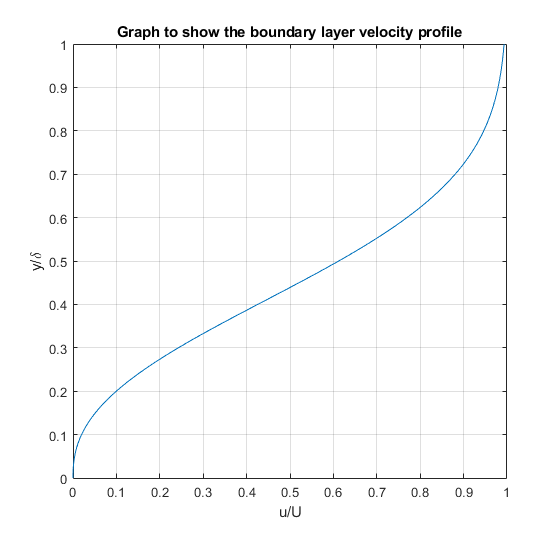
\includegraphics[height = 8cm]{./img/q3a.png}
    \caption{Graph to show boundary layer velocity profile.}
    \label{fig:q3a}
\end{figure}
\end{document}